\documentclass[11pt,a4paper]{article}

\usepackage[T1]{fontenc}
\usepackage[utf8]{inputenc}
\usepackage{mathptmx}
\usepackage[margin=2cm]{geometry}
\usepackage{amsmath}
\usepackage{siunitx}
\usepackage{booktabs}
\usepackage{longtable}
\usepackage{tikz}
\usetikzlibrary{arrows.meta,decorations.pathmorphing,calc,positioning,decorations.pathreplacing}

\sisetup{per-mode = symbol}

% Farben dezent. Die Unterscheidung traegt die Beschriftung, nicht die Farbe,
% damit auch der Schwarzweissdruck lesbar bleibt.
\definecolor{c1}{RGB}{190,110,0}
\definecolor{c2}{RGB}{0,100,150}
\definecolor{c3}{RGB}{0,130,70}
\definecolor{c4}{RGB}{150,50,130}

\newcommand{\Tm}{T_{\mathrm{m}}}
\newcommand{\Cm}{C_{\mathrm{m}}}
\newcommand{\Ta}{T_{\mathrm{a}}}

\pagestyle{empty}
\setlength{\parindent}{0pt}

\begin{document}

%=====================================================================
% SEITE 1
%=====================================================================

{\large\bfseries Thermisches Modell des PV-Moduls: die vier Terme der Energiebilanz}

\vspace{0.8ex}
VU Kontinuierliche Simulation, Projekt PV-Modellierung. Arbeitsblatt für die Startsitzung.

\vspace{1ex}

\begin{center}
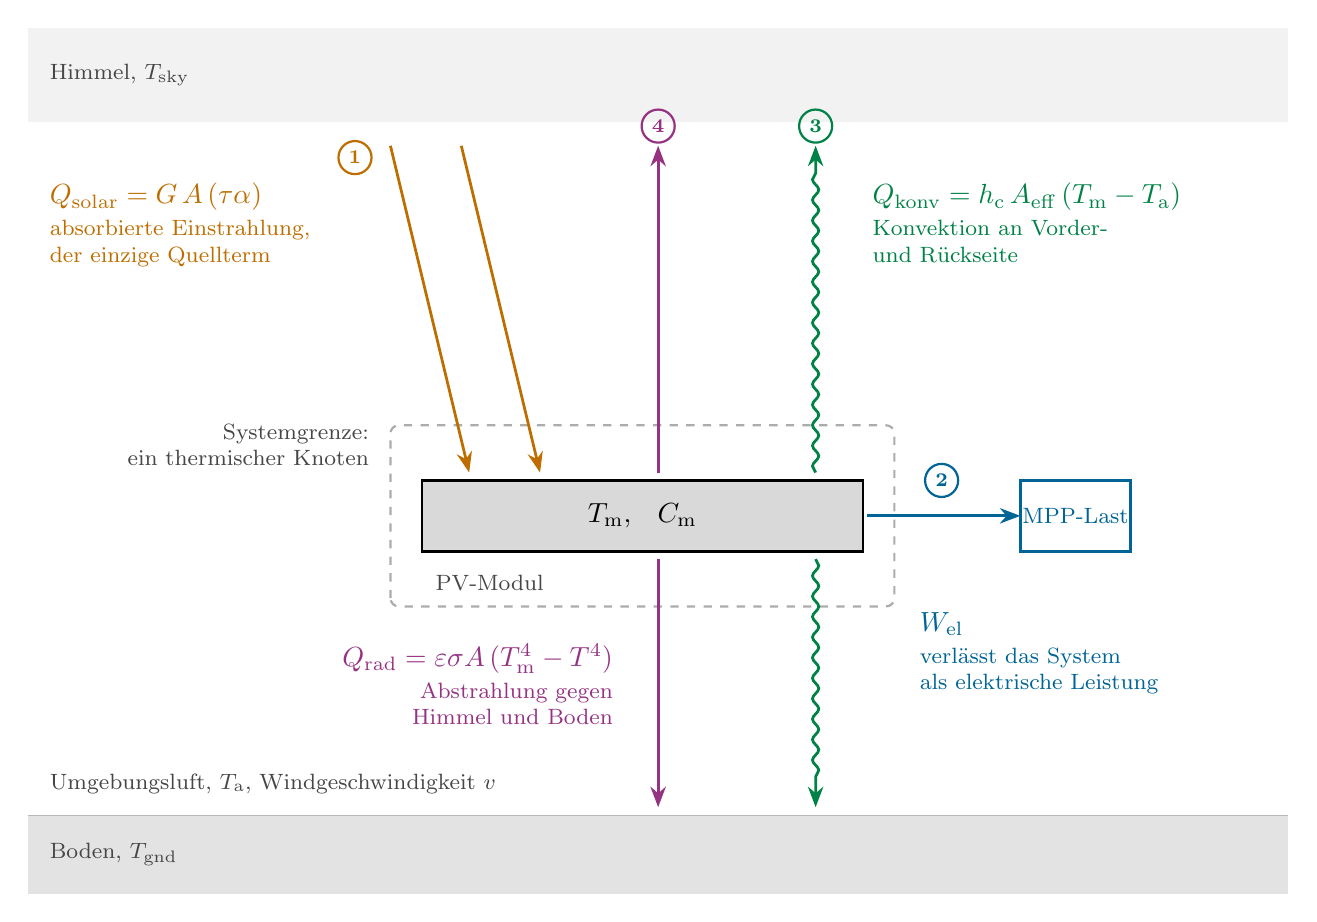
\begin{tikzpicture}[
  font=\footnotesize,
  pfeil/.style={-{Stealth[length=2.6mm]}, line width=1pt},
  welle/.style={-{Stealth[length=2.6mm]}, line width=1pt,
                decorate, decoration={snake, amplitude=0.4mm,
                segment length=2.6mm, post length=2.6mm}},
  nr/.style={circle, draw, line width=0.8pt, inner sep=1pt,
             minimum size=4.2mm, font=\scriptsize\bfseries}
]

% ---------- Himmel, Luft, Boden ----------------------------------
\fill[gray!10] (0,5.0) rectangle (16,6.2);
\node[anchor=west, gray!55!black] at (0.15,5.6) {Himmel, $T_{\mathrm{sky}}$};

\fill[gray!22] (0,-4.8) rectangle (16,-3.8);
\draw[gray!55] (0,-3.8) -- (16,-3.8);
\node[anchor=west, gray!55!black] at (0.15,-4.3) {Boden, $T_{\mathrm{gnd}}$};

\node[anchor=west, gray!55!black] at (0.15,-3.4)
  {Umgebungsluft, $\Ta$, Windgeschwindigkeit $v$};

% ---------- Systemgrenze und Modul -------------------------------
\draw[dashed, gray!65, line width=0.8pt, rounded corners=3pt]
  (4.6,-1.15) rectangle (11.0,1.15);
\node[anchor=east, gray!55!black, align=right] at (4.45,0.9)
  {Systemgrenze:\\ ein thermischer Knoten};

\fill[gray!30] (5.0,-0.45) rectangle (10.6,0.45);
\draw[line width=1pt] (5.0,-0.45) rectangle (10.6,0.45);
\node at (7.8,0.0) {\normalsize $\Tm$, \; $\Cm$};
\node[anchor=west, gray!55!black] at (5.05,-0.85) {PV-Modul};

% ---------- 1) Q_solar: schraege Pfeile von oben -----------------
\draw[pfeil, c1] (4.6,4.7) -- (5.6,0.55);
\draw[pfeil, c1] (5.5,4.7) -- (6.5,0.55);
\node[nr, c1] at (4.15,4.55) {1};
\node[c1, anchor=north west, align=left] at (0.15,4.35)
  {\normalsize $Q_{\mathrm{solar}} = G\,A\,(\tau\alpha)$\\[0.6ex]
   absorbierte Einstrahlung,\\ der einzige Quellterm};

% ---------- 4) Q_rad: senkrecht oben und unten -------------------
\draw[pfeil, c4] (8.0,0.55) -- (8.0,4.7);
\draw[pfeil, c4] (8.0,-0.55) -- (8.0,-3.7);
\node[nr, c4] at (8.0,4.95) {4};
\node[c4, anchor=north east, align=right] at (7.55,-1.5)
  {\normalsize $Q_{\mathrm{rad}} = \varepsilon\sigma A\,(\Tm^4 - T^4)$\\[0.6ex]
   Abstrahlung gegen\\ Himmel und Boden};

% ---------- 3) Q_konv: gewellt oben und unten --------------------
\draw[welle, c3] (10.0,0.55) -- (10.0,4.7);
\draw[welle, c3] (10.0,-0.55) -- (10.0,-3.7);
\node[nr, c3] at (10.0,4.95) {3};
\node[c3, anchor=north west, align=left] at (10.6,4.35)
  {\normalsize $Q_{\mathrm{konv}} = h_{\mathrm{c}}\,A_{\mathrm{eff}}\,(\Tm - \Ta)$\\[0.6ex]
   Konvektion an Vorder-\\ und Rückseite};

% ---------- 2) W_el: nach rechts heraus --------------------------
\draw[pfeil, c2] (10.65,0.0) -- (12.6,0.0);
\draw[c2, line width=1pt] (12.6,-0.45) rectangle (14.0,0.45);
\node[c2] at (13.3,0.0) {MPP-Last};
\node[nr, c2] at (11.6,0.45) {2};
\node[c2, anchor=north west, align=left] at (11.2,-1.1)
  {\normalsize $W_{\mathrm{el}}$\\[0.6ex]
   verlässt das System\\ als elektrische Leistung};

\end{tikzpicture}
\end{center}

\vspace{0.5ex}

\begin{center}
\fbox{\parbox{0.9\textwidth}{\vspace{0.8ex}
\begin{equation*}
  \underbrace{\Cm \frac{\mathrm{d}\Tm}{\mathrm{d}t}}_{\text{Speicherung}}
  \;=\;
  \underbrace{\textcolor{c1}{Q_{\mathrm{solar}}}}_{\textcolor{c1}{\text{\bfseries 1}}}
  \;-\;
  \underbrace{\textcolor{c2}{W_{\mathrm{el}}}}_{\textcolor{c2}{\text{\bfseries 2}}}
  \;-\;
  \underbrace{\textcolor{c3}{Q_{\mathrm{konv}}}}_{\textcolor{c3}{\text{\bfseries 3}}}
  \;-\;
  \underbrace{\textcolor{c4}{Q_{\mathrm{rad}}}}_{\textcolor{c4}{\text{\bfseries 4}}}
\end{equation*}
\vspace{-1.5ex}}}
\end{center}

\vspace{1.5ex}

Ein einziger Energiespeicher im System, also genau ein Zustand: die Modultemperatur
$\Tm$. Daraus folgt eine gewöhnliche Differentialgleichung erster Ordnung.
Nichtlinear ist sie aus zwei Gründen: der $T^4$-Term der Abstrahlung und die
Temperaturabhängigkeit von $W_{\mathrm{el}}$.

\newpage

%=====================================================================
% SEITE 2
%=====================================================================

{\large\bfseries Die vier Terme ausgeschrieben}

\vspace{2ex}

\textcolor{c1}{\bfseries 1\quad Absorbierte Einstrahlung}
\begin{equation*}
  Q_{\mathrm{solar}} = G \cdot A \cdot (\tau\alpha)
\end{equation*}
Der einzige Term mit positivem Vorzeichen. $G$ ist eine Messgröße und treibt das
gesamte System an.

\vspace{2ex}
\textcolor{c2}{\bfseries 2\quad Abgeführte elektrische Leistung}
\begin{equation*}
  W_{\mathrm{el}} = G \cdot A \cdot (\tau\alpha) \cdot \eta_{\mathrm{ref}}
  \left[1 - \beta_{\mathrm{ref}}\left(\Tm - T_{\mathrm{ref}}\right)\right]
\end{equation*}
Diese Energie verlässt das Modul als Strom und wird deshalb nicht zu Wärme. Hier
steht $\Tm$ auf der rechten Seite, das ist die Rückkopplung, die aus einer Bilanz
erst ein dynamisches System macht. Gilt nur im MPP-Betrieb. Im Leerlauf entfällt
der Term und alles wird zu Wärme.

\vspace{2ex}
\textcolor{c3}{\bfseries 3\quad Konvektion}
\begin{equation*}
  Q_{\mathrm{konv}} = h_{\mathrm{c}} \cdot A_{\mathrm{eff}}
  \cdot \left(\Tm - \Ta\right),
  \qquad
  h_{\mathrm{c}} = a + b\,v
\end{equation*}
Der Ansatz für $h_{\mathrm{c}}$ ist eine Entscheidung, keine Naturkonstante. Die
lineare Windkorrelation ist die einfache Variante, die Alternative ist der
Nusselt-Ansatz mit mehreren Strömungsregimen nach Herteleer. Beides gehört in die
Annahmenliste.

\vspace{2ex}
\textcolor{c4}{\bfseries 4\quad Abstrahlung}
\begin{equation*}
  Q_{\mathrm{rad}} = \varepsilon\,\sigma\,A\,F_{\mathrm{sky}}
  \left(\Tm^4 - T_{\mathrm{sky}}^4\right)
  + \varepsilon\,\sigma\,A\,F_{\mathrm{gnd}}
  \left(\Tm^4 - T_{\mathrm{gnd}}^4\right)
\end{equation*}
Zwei Anteile mit derselben Physik und denselben Parametern. $T_{\mathrm{sky}}$ wird
nicht gemessen und muss aus $\Ta$ abgeschätzt werden, üblich nach Swinbank. Bei
horizontaler Montage ist $F_{\mathrm{sky}} \approx 1$ und der Bodenanteil klein,
bei Neigung $\vartheta$ gilt $F_{\mathrm{sky}} = (1+\cos\vartheta)/2$.

\vspace{3ex}
{\bfseries Die Wärmekapazität} folgt aus dem Schichtaufbau des Laminats:
\begin{equation*}
  \Cm = A \sum_i \rho_i\, c_i\, d_i
\end{equation*}

\vspace{1ex}
\begin{center}
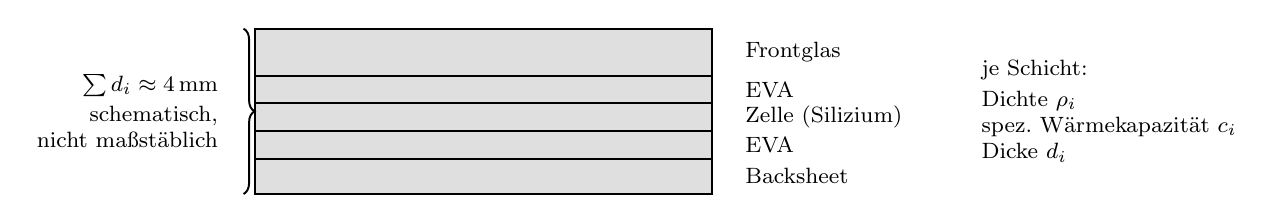
\begin{tikzpicture}[font=\footnotesize]
  \def\xa{2.2} \def\xb{8.0}
  \foreach \y/\h/\name in {
      0.80/0.45/{Backsheet},
      1.25/0.35/{EVA},
      1.60/0.35/{Zelle (Silizium)},
      1.95/0.35/{EVA},
      2.30/0.60/{Frontglas}} {
    \fill[gray!25] (\xa,\y) rectangle (\xb,\y+\h);
    \draw[line width=0.7pt] (\xa,\y) rectangle (\xb,\y+\h);
    \node[anchor=west] at (\xb+0.3,\y+\h/2) {\name};
  }
  \draw[decorate, decoration={brace, amplitude=4pt}, line width=0.7pt]
    (2.05,2.90) -- (2.05,0.80);
  \node[anchor=east, align=right] at (1.85,1.85)
    {$\textstyle\sum d_i \approx \SI{4}{\milli\metre}$\\[0.4ex] schematisch,\\ nicht maßstäblich};
  \node[anchor=west, align=left] at (11.3,1.85)
    {je Schicht:\\[0.4ex] Dichte $\rho_i$\\ spez.\ Wärmekapazität $c_i$\\ Dicke $d_i$};
\end{tikzpicture}
\end{center}

\vspace{1ex}
Alle Schichten haben dieselbe Temperatur $\Tm$. Das ist die zentrale Vereinfachung
und der Grund, warum die Wärmeleitung im Modul gar nicht erst auftaucht. Begründung
für das Protokoll: bei rund \SI{4}{\milli\metre} Gesamtdicke sind die
Temperaturgradienten quer durch das Laminat gegenüber den Unterschieden zur
Umgebung vernachlässigbar.

\newpage

%=====================================================================
% SEITE 3
%=====================================================================

{\large\bfseries Alle Symbole, Einheiten und woher die Werte kommen}

\vspace{1ex}
Die Spalte \emph{Herkunft} ist zugleich die Arbeitsliste für die Parameterrecherche
in Aufgabenpunkt~3. Alles in SI-Einheiten, Temperaturen durchgehend in Kelvin.

\vspace{2ex}

\begin{longtable}{l l l p{0.38\textwidth}}
\toprule
Symbol & Bedeutung & Einheit & Herkunft \\
\midrule
\endhead

\multicolumn{4}{l}{\textit{Zustand und linke Seite der Gleichung}} \\
\addlinespace[0.4ex]
$\Tm$ & Modultemperatur & \si{\kelvin} & Ergebnis der Simulation \\
$\Cm$ & Wärmekapazität des Moduls & \si{\joule\per\kelvin} & berechnet aus Schichtaufbau \\
$t$ & Zeit & \si{\second} & \\
$\rho_i$ & Dichte der Schicht $i$ & \si{\kilogram\per\cubic\metre} & Literatur \\
$c_i$ & spez.\ Wärmekapazität Schicht $i$ & \si{\joule\per\kilogram\per\kelvin} & Literatur \\
$d_i$ & Dicke der Schicht $i$ & \si{\metre} & Datenblatt, Literatur \\
\addlinespace[1ex]

\multicolumn{4}{l}{\textcolor{c1}{\textit{Term 1: absorbierte Einstrahlung}}} \\
\addlinespace[0.4ex]
$G$ & Globalstrahlung in Modulebene & \si{\watt\per\square\metre} & Messdaten GeoSphere, Paperdaten \\
$A$ & Modulfläche & \si{\square\metre} & Datenblatt \\
$\tau$ & Transmissionsgrad Frontglas & -- & Literatur \\
$\alpha$ & Absorptionsgrad der Zelle & -- & Literatur \\
$(\tau\alpha)$ & effektives Produkt & -- & Literatur, Größenordnung $0{,}9$ \\
\addlinespace[1ex]

\multicolumn{4}{l}{\textcolor{c2}{\textit{Term 2: elektrische Leistung}}} \\
\addlinespace[0.4ex]
$W_{\mathrm{el}}$ & abgeführte elektrische Leistung & \si{\watt} & berechnet \\
$\eta_{\mathrm{ref}}$ & Wirkungsgrad bei STC & -- & Datenblatt \\
$\beta_{\mathrm{ref}}$ & Temperaturkoeffizient der Leistung & \si{\per\kelvin} & Datenblatt, Größenordnung $0{,}004$ \\
$T_{\mathrm{ref}}$ & Referenztemperatur (STC) & \si{\kelvin} & Norm, $\SI{298.15}{\kelvin}$ \\
\addlinespace[1ex]

\multicolumn{4}{l}{\textcolor{c3}{\textit{Term 3: Konvektion}}} \\
\addlinespace[0.4ex]
$h_{\mathrm{c}}$ & Wärmeübergangskoeffizient & \si{\watt\per\square\metre\per\kelvin} & Korrelation, Entscheidung der Gruppe \\
$A_{\mathrm{eff}}$ & wirksame Fläche & \si{\square\metre} & Annahme, meist $2A$ \\
$\Ta$ & Umgebungslufttemperatur & \si{\kelvin} & Messdaten; Annahme bei der Validierung \\
$v$ & Windgeschwindigkeit & \si{\metre\per\second} & Messdaten GeoSphere \\
$a$, $b$ & Koeffizienten der Windkorrelation & \si{\watt\per\square\metre\per\kelvin} & Literatur \\
\addlinespace[1ex]

\multicolumn{4}{l}{\textcolor{c4}{\textit{Term 4: Abstrahlung}}} \\
\addlinespace[0.4ex]
$\varepsilon$ & Emissivität der Oberfläche & -- & Literatur, $0{,}85$ bis $0{,}9$ \\
$\sigma$ & Stefan-Boltzmann-Konstante & \si{\watt\per\square\metre\per\kelvin\tothe{4}} & Naturkonstante, $\num{5.670e-8}$ \\
$T_{\mathrm{sky}}$ & Himmelstemperatur & \si{\kelvin} & berechnet aus $\Ta$, z.\,B.\ nach Swinbank \\
$T_{\mathrm{gnd}}$ & Bodentemperatur & \si{\kelvin} & Annahme, häufig $\Ta$ \\
$F_{\mathrm{sky}}$, $F_{\mathrm{gnd}}$ & Sichtfaktoren & -- & Geometrie, aus dem Neigungswinkel \\
$\vartheta$ & Neigungswinkel des Moduls & \si{\degree} & Angabe der Messkampagne \\
\bottomrule
\end{longtable}

\newpage

%=====================================================================
% SEITE 4
%=====================================================================

{\large\bfseries Dieselbe Gleichung als Blockdiagramm}

\vspace{1ex}
Ein Zustand, also genau ein Integrator. Diese Struktur bauen wir in Aufgabenpunkt~7
in SIMULINK nach, in MATLAB übernimmt der ODE-Solver die Integration.

\vspace{3ex}

\begin{center}
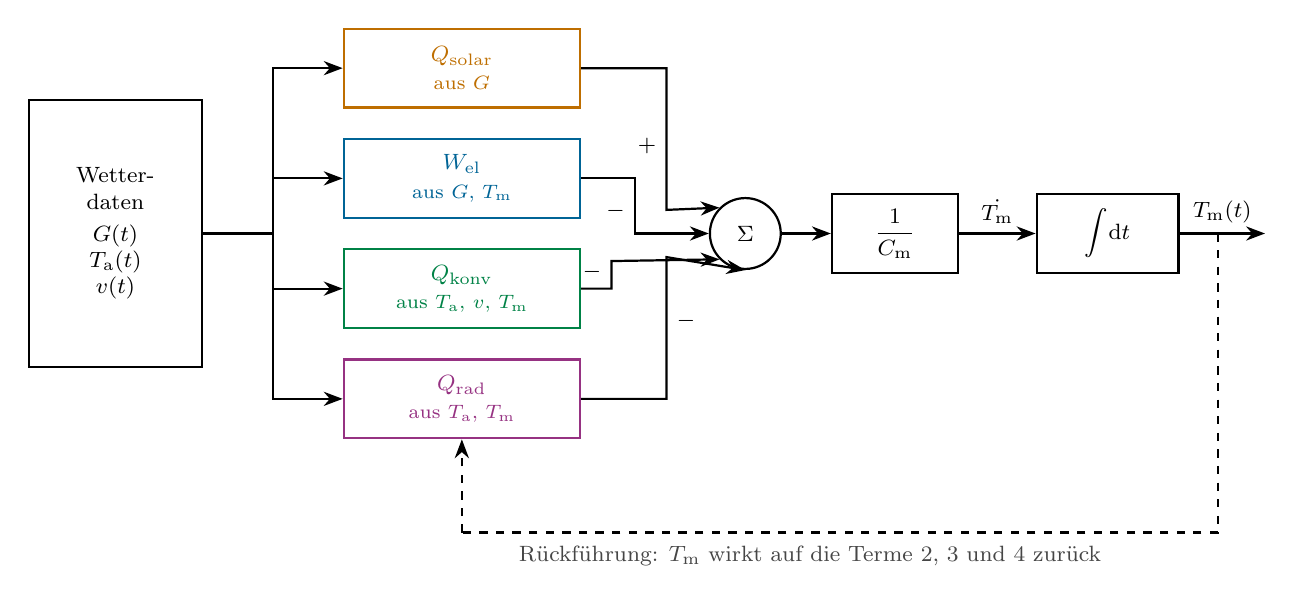
\begin{tikzpicture}[
  font=\footnotesize,
  blk/.style={draw, line width=0.8pt, minimum width=3.0cm, minimum height=1.0cm,
              align=center},
  sum/.style={draw, line width=0.8pt, circle, minimum size=0.9cm, inner sep=0pt},
  pf/.style={-{Stealth[length=2.4mm]}, line width=0.8pt}
]

% Wetterdaten
\node[blk, minimum width=2.2cm, minimum height=3.4cm, align=center]
  (wet) at (0.0,0.6) {Wetter-\\daten\\[0.6ex] $G(t)$\\ $\Ta(t)$\\ $v(t)$};

% Termbloecke
\node[blk, draw=c1, text=c1] (b1) at (4.4,2.7)  {$Q_{\mathrm{solar}}$\\[0.2ex] {\scriptsize aus $G$}};
\node[blk, draw=c2, text=c2] (b2) at (4.4,1.3)  {$W_{\mathrm{el}}$\\[0.2ex] {\scriptsize aus $G$, $\Tm$}};
\node[blk, draw=c3, text=c3] (b3) at (4.4,-0.1) {$Q_{\mathrm{konv}}$\\[0.2ex] {\scriptsize aus $\Ta$, $v$, $\Tm$}};
\node[blk, draw=c4, text=c4] (b4) at (4.4,-1.5) {$Q_{\mathrm{rad}}$\\[0.2ex] {\scriptsize aus $\Ta$, $\Tm$}};

\draw[pf] (wet.east) -- (2.0,0.6) -- (2.0,2.7) -- (b1.west);
\draw[pf] (2.0,0.6) -- (2.0,1.3) -- (b2.west);
\draw[pf] (2.0,0.6) -- (2.0,-0.1) -- (b3.west);
\draw[pf] (2.0,0.6) -- (2.0,-1.5) -- (b4.west);

% Summierer
\node[sum] (s) at (8.0,0.6) {$\Sigma$};
\draw[pf] (b1.east) -- (7.0,2.7)  -- node[pos=0.55, left] {$+$} (7.0,0.9) -- (s.north west);
\draw[pf] (b2.east) -- (6.6,1.3)  -- node[pos=0.6, left] {$-$} (6.6,0.6) -- (s.west);
\draw[pf] (b3.east) -- (6.3,-0.1) -- node[pos=0.6, left] {$-$} (6.3,0.25) -- (s.south west);
\draw[pf] (b4.east) -- (7.0,-1.5) -- node[pos=0.55, right] {$-$} (7.0,0.3) -- (s.south);

% Verstaerkung und Integrator
\node[blk, minimum width=1.6cm] (gain) at (9.9,0.6) {$\dfrac{1}{\Cm}$};
\node[blk, minimum width=1.8cm] (int)  at (12.6,0.6) {$\displaystyle\int\!\mathrm{d}t$};
\draw[pf] (s.east) -- (gain.west);
\draw[pf] (gain.east) -- node[above] {$\dot{\Tm}$} (int.west);
\draw[pf] (int.east) -- node[above] {$\Tm(t)$} (14.6,0.6);

% Rueckfuehrung
\draw[dashed, line width=0.9pt] (14.0,0.6) -- (14.0,-3.2) -- (4.4,-3.2);
\draw[pf, dashed, line width=0.9pt] (4.4,-3.2) -- (b4.south);
\node[anchor=west, gray!55!black] at (5.0,-3.5)
  {Rückführung: $\Tm$ wirkt auf die Terme 2, 3 und 4 zurück};

\end{tikzpicture}
\end{center}

\vspace{4ex}

Die Rückführung ist der eigentliche Grund, warum das Modell simuliert werden muss
und nicht in einer Formel auflösbar ist. $\Tm$ wirkt auf den Wirkungsgrad, auf den
Konvektions- und auf den Strahlungsterm zurück.

\vspace{4ex}
{\footnotesize Arbeitsgrundlage für die Startsitzung. Die genannten Zahlenwerte sind
Größenordnungen zur Orientierung und ersetzen die Literaturrecherche nicht.}

\end{document}
